\documentclass[aspectratio=169,t]{beamer}

\usepackage{blindtext}

\usetheme{Execushares}

\title{Formal Methods to the Rescue? Experiences Coding in a Theorem Prover}
\subtitle{\url{https://github.com/diekmann/} \  @popitter\_net}
\author{Cornelius Diekmann}
\date{April 9, 2018}

\setcounter{showSlideNumbers}{1}



\usepackage{tikzsymbols} %\Snowman
\mathchardef\mhyphen="2D % Define a "math hyphen"
\usepackage{fancyvrb}


\usetikzlibrary{shapes}
\usetikzlibrary{calc}
%\usetikzlibrary{decorations}
\usetikzlibrary{arrows,decorations.markings}
%this should make nicer arrows simpler:
%requires at least TikZ 3.0.0!
%\usetikzlibrary{arrows.meta}
\usetikzlibrary{arrows.meta} %need pgf > 3.0.
\tikzset{myptr/.style={-{Latex[scale=2.5]}}}

\tikzset{every loop/.style={min distance=10mm,looseness=10}}



\newcommand{\hairspace}{\hspace{1pt}}
\newcommand{\eg}{\mbox{e.\hairspace{}g.,} }
\newcommand{\ie}{\mbox{i.\hairspace{}e.,} }
\newcommand{\Ie}{\mbox{I.\hairspace{}e.,} }
\newcommand{\cf}{\mbox{cf.}\ }
\newcommand{\etal}{\mbox{et~al.}\ }

\usepackage{fancyvrb}

\usepackage{IEEEtrantools}

%https://tex.stackexchange.com/questions/220820/itemize-list-inside-a-tikzpicture-node
\usepackage{varwidth}

% math typesetting
% free variables
\newcommand{\mvar}[1]{\ensuremath{\mathit{#1}}}
% definitions and constants
\newcommand{\mdef}[1]{\ensuremath{\mathsf{#1}}}
% executable functions
\newcommand{\mfun}[1]{\mdef{#1}}
%datatype constructor (may appear in text)
\newcommand\mconstr[1]{\mdef{#1}}
%math control (if then else)
\newcommand\mctrl[1]{\ensuremath{\mathbf{#1}}}


\newcommand{\BigO}{\mathcal{O}}


\DeclareMathSymbol{\mlq}{\mathord}{operators}{``}
\DeclareMathSymbol{\mrq}{\mathord}{operators}{`'}


\newcommand\mdoubleplus{\ensuremath{\mathbin{+\mkern-10mu+}}}
\newcommand\lstapp{\ensuremath{\mathbin{:\mkern-1mu:\mkern-1mu:}}} %list append
\newcommand\lstcons{\ensuremath{\mathbin{:\mkern-1mu:}}} %list append


\newcommand{\free}[1]{\textcolor{DarkerBlue}{#1}}
\newcommand{\bound}[1]{\textcolor{DarkGreen}{#1}}
%\newcommand{\boundi}[1]{\textcolor{Green}{#1}}


\newcommand*\circled[1]{\tikz[baseline=-3pt, scale=0.5, every node/.style={scale=0.5}]{\node[shape=circle,draw,inner sep=1pt,minimum size=16pt] (char) {#1};}}

\newcommand\allow{\ensuremath{\textnormal{\circled{\large \textbf{\checkmark}}}}}
\newcommand\deny{\ensuremath{\textnormal{\circled{\large \textbf{\texttimes}}}}}
\newcommand\undecided{\ensuremath{\textnormal{\circled{\textnormal{\large \textbf{?}}}}}}

\newcommand\matchop[1]{\ensuremath{\mfun{match}\ {#1}}}
\newcommand\matches[1]{\ensuremath{\matchop\gamma \ #1 \ p}}
\newcommand\nmatches[1]{\ensuremath{\neg\; \matchop\gamma \ #1 \ p}}
\newcommand\bigstep[5]{\ensuremath{\free{\Gamma},#1,#2 \vdash\big\langle #3,\; #4 \big\rangle \Rightarrow #5}}





%%%http://tex.stackexchange.com/questions/75120/how-to-make-highlighting-work-in-beamer-with-overlays

%\usepackage{xcolor}

%  http://tex.stackexchange.com/questions/46434/how-to-highlight-text-formals-with-tikz
\usepackage{tikz}
\makeatletter
%
% Highlighter code
%

\tikzset{%
  remember picture with id/.style={%
    remember picture,
    overlay,
    save picture id=#1,
  },
  save picture id/.code={%
    \edef\pgf@temp{#1}%
    \immediate\write\pgfutil@auxout{%
      \noexpand\savepointas{\pgf@temp}{\pgfpictureid}}%
  }
}

\def\savepointas#1#2{%
  \expandafter\gdef\csname save@pt@#1\endcsname{#2}%
}

\tikzdeclarecoordinatesystem{pic}{%
  \@ifundefined{save@pt@#1}{%
    \pgfpointorigin
  }{%
  \pgfsys@getposition{\csname save@pt@#1\endcsname}\save@orig@pic%
  \pgfsys@getposition{\pgfpictureid}\save@this@pic%
  \pgf@process{\pgfpointorigin\save@this@pic}%
  \pgf@xa=\pgf@x
  \pgf@ya=\pgf@y
  \pgf@process{\pgfpointorigin\save@orig@pic}%
  \advance\pgf@x by -\pgf@xa
  \advance\pgf@y by -\pgf@ya
  }%
}

\newcounter{highlight}
\newcommand{\hlstart}{\tikz[remember picture with id=hlstart\the\value{highlight},baseline=-0.7ex];\hl@start}
\newcommand{\hlend}{\tikz[remember picture with id=hlend\the\value{highlight},baseline=-0.7ex];\hl@end\stepcounter{highlight}}
\newcommand{\fdstart}{\tikz[remember picture with id=hlstart\the\value{highlight},baseline=-0.7ex];\fd@start}
\newcommand{\fdend}{\tikz[remember picture with id=hlend\the\value{highlight},baseline=-0.7ex];\fd@end\stepcounter{highlight}}
\newcommand{\vlstart}{\tikz[remember picture with id=hlstart\the\value{highlight},baseline=-1em];\vl@start}
\newcommand{\vlend}{\tikz[remember picture with id=hlend\the\value{highlight},baseline=0.3ex];\vl@end\stepcounter{highlight}}

\newcommand{\hl@start}[1][]{%
  \hl@draw{highlighter}{#1}{\the\value{highlight}}}

\newcommand{\hl@end}{}

\newcommand{\fd@start}[1][]{%
  \def\fd@args{#1}}

\newcommand{\fd@end}{\def\@tempa{\hl@draw{fader}}\expandafter\@tempa\expandafter{\fd@args}{\the\value{highlight}}\def\fd@args{}}

\newcommand{\vl@start}[1][]{%
  \vl@draw{highlighter}{#1}{\the\value{highlight}}}

\newcommand{\vl@end}{}


\def\hl@sets{%
  \edef\hl@sx{\the\pgf@x}%
  \edef\hl@sy{\the\pgf@y}%
}
\def\hl@sete{%
  \edef\hl@ex{\the\pgf@x}%
  \edef\hl@ey{\the\pgf@y}%
}

\@ifclassloaded{beamer}{

\def\page@node{
  \path (current page.south east)
      ++(-\beamer@rightmargin,\footheight)
  node[
    minimum width=\textwidth,
    minimum height=\textheight,
    anchor=south east
  ] (page) {};
}

}{

  \def\page@node{
    \path (current page.north west)
    ++(\hoffset + 1in + \oddsidemargin + \leftskip,\voffset + 1in + \topmargin + \headheight + \headsep)
    node[
      minimum width=\textwidth - \leftskip - \rightskip,
      minimum height=\textheight,
      anchor=north west
    ] (page) {};
  }

}

\newcommand{\hl@draw}[3]{%
  \begin{tikzpicture}[remember picture,overlay]%
  \page@node
  \tikzset{#2,highlight=#1,every path/.append style={highlight=#1}}%
  \pgfmathsetlengthmacro{\hl@width}{\the\pgflinewidth - 1pt}%
  \coordinate (hlstart) at (pic cs:hlstart#3);
  \coordinate (hlend) at (pic cs:hlend#3);
  \tikz@scan@one@point\hl@sets(pic cs:hlstart#3)
  \tikz@scan@one@point\hl@sete(pic cs:hlend#3)
  \ifdim\hl@sy=\hl@ey\relax
  \draw (hlstart) -- (hlend);
  \else
  \draw (hlstart) -- (hlstart -| page.east);
  \pgfmathsetlengthmacro{\hl@sy}{\hl@sy -\hl@width}%
  \pgfmathsetlengthmacro{\hl@ey}{\hl@ey +\hl@width}%
  \loop\ifdim\hl@sy>\hl@ey\relax
  \draw (0,\hl@sy -| page.west) -- (0,\hl@sy -| page.east);
  \pgfmathsetlengthmacro{\hl@sy}{\hl@sy -\hl@width}%
  \repeat
  \draw (hlend -| page.west) -- (hlend);
  \fi
  \end{tikzpicture}%
}

\newcommand{\vl@draw}[3]{%
  \begin{tikzpicture}[remember picture,overlay]%
  \page@node
  \tikzset{#2,highlight=#1,every path/.append style={highlight=#1}}%
  \pgfmathsetlengthmacro{\hl@width}{\the\pgflinewidth - 1pt}%
  \coordinate (hlstart) at (pic cs:hlstart#3);
  \coordinate (hlend) at (pic cs:hlend#3);
  \tikz@scan@one@point\hl@sets(pic cs:hlstart#3)
  \tikz@scan@one@point\hl@sete(pic cs:hlend#3)
  \ifdim\hl@sx=\hl@ex\relax
  \draw (hlstart) -- (hlend);
  \else
  \draw (hlstart) -- (hlstart |- page.south);
  \pgfmathsetlengthmacro{\hl@sx}{\hl@sx -\hl@width}%
  \pgfmathsetlengthmacro{\hl@ex}{\hl@ex +\hl@width}%
  \loop\ifdim\hl@sx>\hl@ex\relax
  \draw (\hl@sx,0 |- page.north) -- (\hl@sx,0 |- page.south);
  \pgfmathsetlengthmacro{\hl@sx}{\hl@sx -\hl@width}%
  \repeat
  \draw (hlend |- page.north) -- (hlend);
  \fi
  \end{tikzpicture}%
}

\tikzset{%
  highlight/.default=highlighter,
  highlight/.style={
    color=\pgfkeysvalueof{/tikz/#1 colour},
    line width=\pgfkeysvalueof{/tikz/#1 width},
    line cap=\pgfkeysvalueof{/tikz/#1 cap},
    opacity=\pgfkeysvalueof{/tikz/#1 opacity},
  },
  highlighter colour/.initial=ExecusharesYellow,
  highlighter width/.initial=10pt,% <-- Tweak (was 12pt)
  highlighter cap/.initial=butt,
  highlighter opacity/.initial=1,
  fader colour/.initial=gray,
  fader width/.initial=12pt,
  fader cap/.initial=butt,
  fader opacity/.initial=.5,
}



\@ifclassloaded{beamer}{

%% Beamer variants

\setbeamercolor{highlighted text}{bg=ExecusharesYellow}
\setbeamercolor{faded text}{fg=gray}

\newcommand<>{\highlight}[2][]{%
  \only#3{\hlstart[#1]}#2\only#3{\hlend}}

\newcommand<>{\fade}[2][]{%
  \only#3{\fdstart[#1]}#2\only#3{\fdend}}

\newcommand<>{\vhighlight}[2][]{%
  \only#3{\vlstart[#1]}#2\only#3{\vlend}}

}{

\newcommand{\highlight}[2][]{%
\hlstart[#1]#2\hlend}

\newcommand{\fade}[2][]{%
\fdstart[#1]#2\fdend}

\newcommand{\vhighlight}[2][]{%
\vlstart[#1]#2\vlend}

}



\begin{document}
\setcounter{showProgressBar}{0}
\setcounter{showSlideNumbers}{0}


\frame{\titlepage}


%\begin{frame}
%	\frametitle{Contents}
%	\begin{enumerate}
%		\item Introduction \\ \textcolor{ExecusharesGrey}{\footnotesize\hspace{1em} The reasoning and background behind this theme}
%		\item Lorem Text  \\ \textcolor{ExecusharesGrey}{\footnotesize\hspace{1em} Just some Lorem Ipsum for filler}
%		\item Conclusions \\ \textcolor{ExecusharesGrey}{\footnotesize\hspace{1em} Some closing thoughts}
%	\end{enumerate}
%\end{frame}


\setcounter{framenumber}{0}
\setcounter{showProgressBar}{1}
\setcounter{showSlideNumbers}{1}


\section{About Me}
\begin{frame}
	\frametitle{About Me}
	\vspace*{5ex}
	\begin{columns}
	\begin{column}{0.5\textwidth}
		\begin{itemize}
			\item I did this work as PhD student at TUM
			\begin{itemize}
				\item Which was awesome!
			\end{itemize}
			\item Now I work at Google
			\begin{itemize}
				\item Which is awesome, too!
				\item This presentation is not related in any way to Google
			\end{itemize}
		\end{itemize}
	\end{column}
	\begin{column}{0.5\textwidth}
	    \begin{center}
	     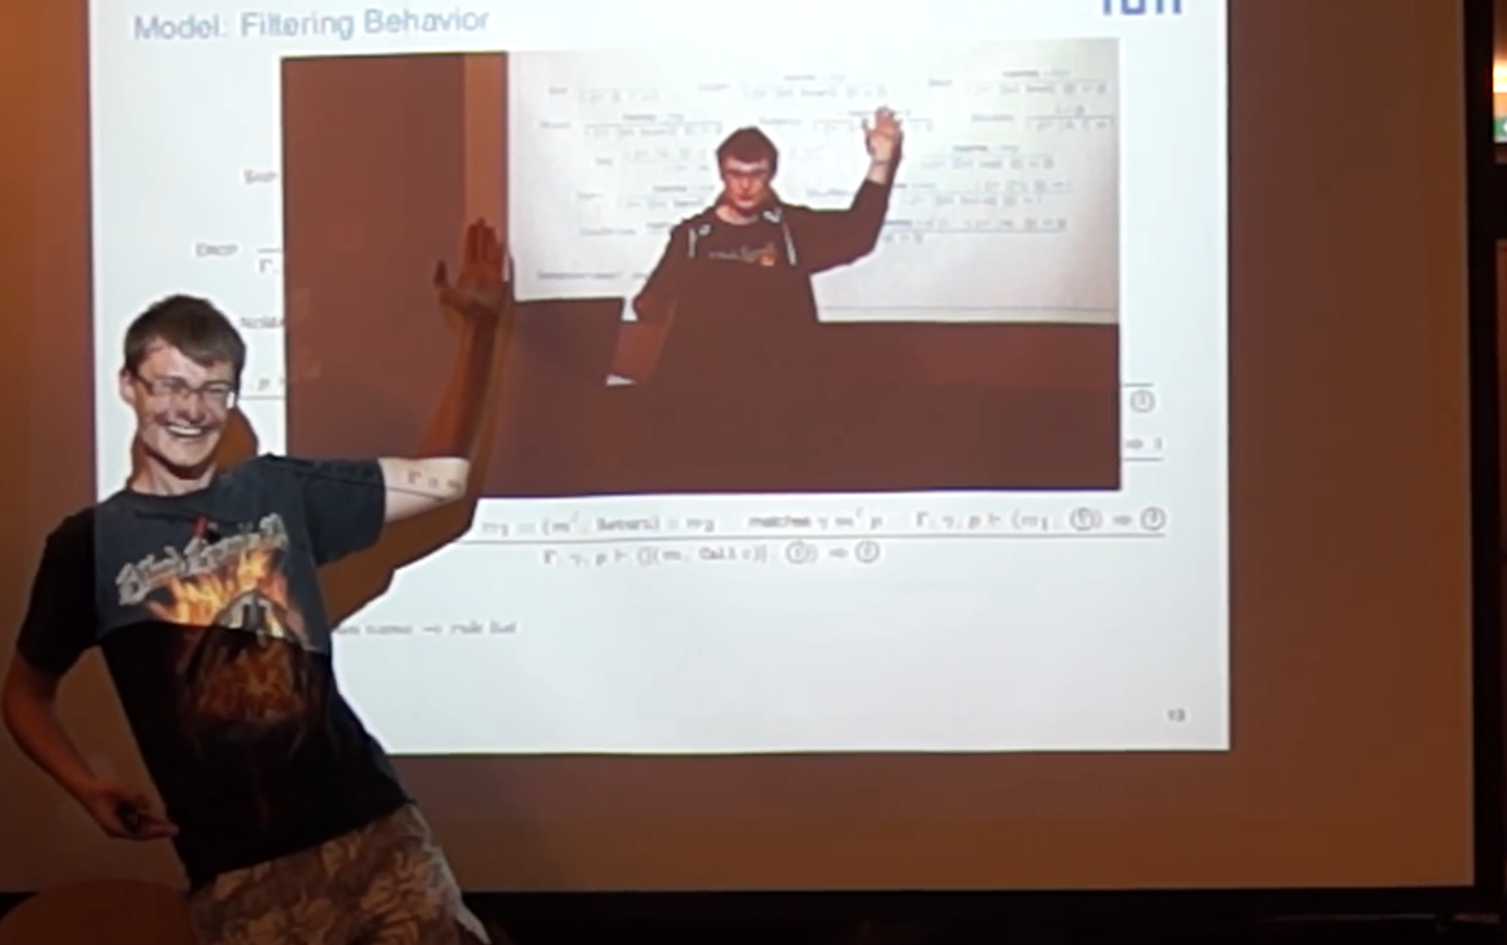
\includegraphics[width=0.99\textwidth]{meta2.png}\\
	     {\scriptsize Fig 1.: Me pointing at slides pointing at slides.}
	     \end{center}
	\end{column}
	\end{columns}
	\bigskip
	\begin{center}
		Thoughts and opinions are my own, not those of my company.
	\end{center}
\end{frame}



\section{Linux iptables by Example}

\newcommand{\valert}[2][]{%
  \if\relax\detokenize{#1}\relax% http://tex.stackexchange.com/q/53068/5764
    {#2}% Default overlay
  \else
    \highlight<#1>{#2}% Specific overlay
  \fi}

\begin{frame}[fragile]
	\frametitle{iptables Example}
	\vspace*{4ex}
	
\hskip-1em\begin{minipage}{\linewidth}
%break symbol $\hookleftarrow$
% frame=single,label=Upper Closure
\footnotesize
%:INPUT DROP [0:0]
%:OUTPUT DROP [0:0]
\begin{Verbatim}[commandchars=\\\{\},codes={\catcode`$=3\catcode`^=7}]
*filter
:FORWARD DROP [0:0]
:DOS_PROTECT - [0:0]
:GOOD~STUFF - [0:0]
-A FORWARD -j DOS_PROTECT
-A FORWARD -j GOOD~STUFF
-A FORWARD -p tcp -m multiport ! --dports 80,443,6667,6697 -m hashlimit $\hfill\hookleftarrow$
    --hashlimit-above 10/sec --hashlimit-burst 20 --hashlimit-mode srcip $\hfill\hookleftarrow$
    --hashlimit-name aflood --hashlimit-srcmask 8 -j LOG
-A FORWARD ! -i lo -s 127.0.0.0/8 -j DROP
-A FORWARD -i internal -s 131.159.21.0/24 -j ACCEPT
-A FORWARD -s 131.159.15.240/28 -d 131.159.21.0/24 -j DROP
-A FORWARD -p tcp -d 131.159.15.240/28 -j ACCEPT
\valert[2,3,4,5,6,7]{-A FORWARD -i \textcolor{red}{\Snowman} -p tcp -s 131.159.15.240/28 -j ACCEPT}
-A GOOD~STUFF -i lo -j ACCEPT
-A GOOD~STUFF -m state --state ESTABLISHED -j ACCEPT
-A GOOD~STUFF -p icmp -m state --state RELATED -j ACCEPT
-A DOS_PROTECT -i eth1 -p icmp -m icmp --icmp-type 8 $\dots$ --limit 1/sec -j RETURN
-A DOS_PROTECT -i eth1 -p icmp -m icmp --icmp-type 8 -j DROP
COMMIT
\end{Verbatim}
\end{minipage}%$%stupid texmaker

\begin{tikzpicture}[overlay]
	        %\node<15> (wat) at (current page.center) {\includegraphics[width=.45\linewidth]{wat.png}};
	        %\node<16> (watserverfault) at ($(current page.center) + (0,-2ex)$) {\includegraphics[width=.80\linewidth]{watserverfault.png}};
	        
	        \node<3> (wat) at (current page.center) {\resizebox{.2\textwidth}{!}{\verb~-i~ \textcolor{red}{\Snowman}}};
	        \node<4> (wat) at (current page.center) {\resizebox{.4\textwidth}{!}{\verb~-i~ \textcolor{red}{\Snowman}}};
	        \node<5> (wat) at (current page.center) {\resizebox{.8\textwidth}{!}{\verb~-i~ \textcolor{red}{\Snowman}}};
	        
	        \node<6> (snow1) at ($(current page.center) + (0,-2ex)$) {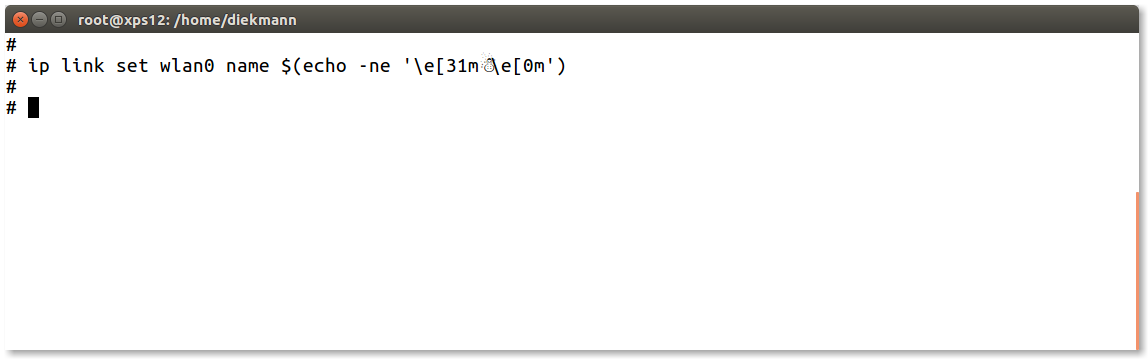
\includegraphics[width=.80\linewidth]{iplink1.png}};
	        \node<7> (snow1) at ($(current page.center) + (0,-2ex)$) {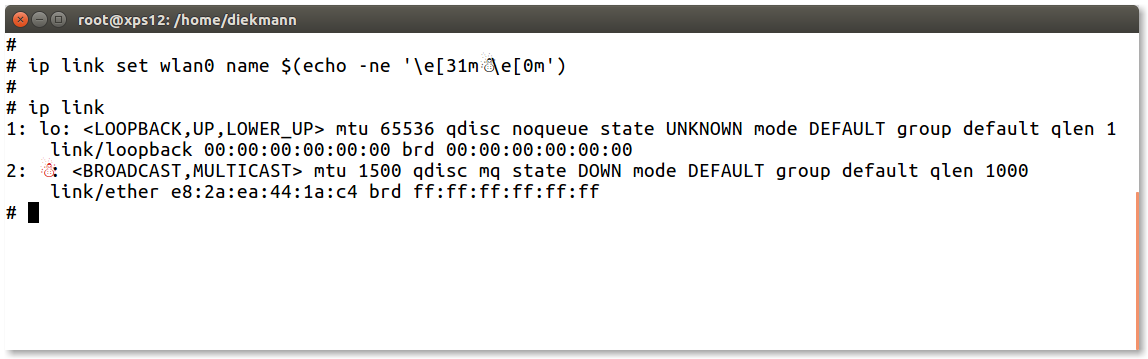
\includegraphics[width=.80\linewidth]{iplink2.png}};
	\end{tikzpicture}
\only<8>{}%force another slide
\end{frame}


\begin{frame}[fragile]
	\frametitle{Visualized for HTTP}

\resizebox{\linewidth}{!}{%
\scriptsize
  \begin{tikzpicture}
	\node[align=center,text width=4cm] (a) at (-4,-3) {\only<1-4>{$131.159.21.0/24$}\only<5->{\begin{large}Internal\end{large}}}; %internal
	\node[align=center,text width=4cm] (b) at (4,-3) {\only<1-5>{$131.159.15.240/28$}\only<6->{\begin{large}DMZ\end{large}}}; %dmz
	\node<1>[align=left] (c) at (0,-4.5) {$127.0.0.0/8$};
	\node[align=center,text width=4cm,cloud, draw,cloud puffs=8,cloud puff arc=120, aspect=2, inner sep=-1.3em,outer sep=0, fill=ExecusharesWhite] (d) at (0,0) {\only<1,2>{$\{0.0.0.0 .. 126.255.255.255\} \cup \{128.0.0.0 .. 131.159.15.239\} \cup \{131.159.16.0 .. 131.159.20.255\} \cup \{131.159.22.0 .. 255.255.255.255\}$}\only<3>{\begin{large}Neuland\end{large}}\only<4->{\begin{large}Internet\end{large}}};
	
	\draw[myptr] (a) to[loop above] (a);
	\draw[myptr] (a) to (b);
	\draw<1>[myptr] (a) to (c);
	\draw[myptr] (a) to (d);
	\draw[myptr] (b) to[loop above] (b);
	\draw<1>[myptr] (b) to (c);
	\draw[myptr] (b) to (d);
	\draw<1>[myptr] (c) to (a);
	\draw<1>[myptr] (c) to (b);
	\draw<1>[myptr] (c) to[loop below] (c);
	\draw<1>[myptr] (c) to (d);
	\draw[myptr] (d) to (b);
  \end{tikzpicture}%
}
\end{frame}


\section{About this Tool}

\begin{frame}
	\frametitle{Bold Claim}
	\vspace*{5ex}
	\begin{itemize}
		\item I coded a tool to print this visualization
		\begin{itemize}
			\item<2-> Okay, TikZ and Graphviz draw the image, but my tool computes the graph
		\end{itemize}
	\end{itemize}
	\onslide<3->{
	\medskip
	\begin{center}
	\begin{Large}
		\alert{If the graph looks good to you, your firewall configuration is secure!}
	\end{Large}
	\end{center}
	}
	\begin{itemize}
		\item<4-> My tool is secure!
		\item<5-> What does this actually mean?
		\begin{itemize}
			\item<6-> It has no errors.
			\item<7-> It does the right thing.
			\item<8-> If it presents you a graph, and you LGTM the graph, the firewall config does the right thing.
		\end{itemize}
	\end{itemize}
\end{frame}


\section{How to Specify Correctness?}

\begin{frame}[fragile]
	\frametitle{Correctness Theorem!}
	\vspace*{5ex}
		Assumes	
    \begin{itemize}
	    \item<1> Unfolded $\free{\mvar{rs}}$ for $\free{\Gamma}$
	    \item<1> $\free{\mvar{p}}$ is \texttt{NEW}% and has \texttt{SYN} set (if TCP)
	    \item \only<1-6>{\highlight<3,4>{$\bigstep{\highlight<5>{\free{\gamma}}}{\free{p}}{\free{\mvar{rs}}}{\undecided}{\allow}$}\qquad} \only<4->{``Firewall with ruleset $\free{\mvar{rs}}$ accepts packet $\free{p}$''}
	    \begin{itemize}
	    	\item<5-> \only<5,6>{$\free{\gamma}$: arbitrary function\qquad}\only<6->{For \emph{all} iptables matching features}
	    \end{itemize}
	    \item Let $(\free{V}, \free{E}) = \mfun{compute\_graph}\ (\mdef{prot}\ \free{p}, \mdef{sport}\ \free{p}, \mdef{dport}\ \free{p})\ (\mfun{simplify}\ \free{\mvar{rs}})$
	    \begin{itemize}
	    	\item $(\mdef{prot}\ \free{p}, \mdef{sport}\ \free{p}, \mdef{dport}\ \free{p})$: Example $(\mvar{tcp},\ 42242,\ 80)$
	    \end{itemize}
    \end{itemize}
    Shows%
    \begin{center}%
	    \vskip-3ex%
	    \begin{overprint}
	    \onslide<1-16>{
        \begin{IEEEeqnarray*}{l}
	    \exists \highlight<13>{\bound{\mvar{s}_\text{repr}}}\ \highlight<13>{\bound{\mvar{d}_\text{repr}}}\ \highlight<14>{\bound{\mvar{s}_\text{range}}}\ \highlight<14>{\bound{\mvar{d}_\text{range}}}.\ \ (\highlight<13>{\bound{\mvar{s}_\text{repr}}}, \highlight<13>{\bound{\mvar{d}_\text{repr}}}) \in  \mdef{set}\ \free{\mvar{E}} \  \wedge  \\
	    \qquad (\mfun{map\_of}\ \free{\mvar{V}})\ \highlight<13>{\bound{\mvar{s}_\text{repr}}} = \mdef{Some}\ \highlight<14>{\bound{\mvar{s}_\text{range}}} \ \wedge \ \highlight<15>{(\mdef{src}\ \free{\mvar{p}}) \in \highlight<14>{\bound{\mvar{s}_\text{range}}}} \ \wedge \\
	    \qquad (\mfun{map\_of}\ \free{\mvar{V}})\ \highlight<13>{\bound{\mvar{d}_\text{repr}}} = \mdef{Some}\ \highlight<14>{\bound{\mvar{d}_\text{range}}} \ \wedge \ \highlight<15>{(\mdef{dst}\ \free{\mvar{p}}) \in \highlight<14>{\bound{\mvar{d}_\text{range}}}}
	    \end{IEEEeqnarray*}}
	    \onslide<17->{In the graph, we can find an arrow from \ $\mdef{src}\ \free{\mvar{p}}$ $\longrightarrow$ $\mdef{dst}\ \free{\mvar{p}}$}
	    
	    \onslide<18->{Warning: The other direction may not hold!}
	    \end{overprint}
    \end{center}
    \medskip
    %Reads: If the firewall accepts a packet, we can look up source and destination IP in the graph.

	% such meta meta!
	\begin{tikzpicture}[overlay]
	    \node<8-11>[fill=white, draw=black, line width=3pt, inner sep=10pt] (tikzmeta) at (current page.center) {\begin{minipage}{.6\linewidth}
\footnotesize
\texttt{\textbackslash{}begin\{tikzpicture\}}\\
\texttt{\hspace*{1ex}\textbackslash{}node (\highlight<9>{a}) at (-4,-4) \{\highlight<10>{\$131.159.21.0/24\$}\};}\\
\texttt{\hspace*{1ex}\textbackslash{}node (b) at (4,-4) \{\$131.159.15.240/28\$\};}\\
\texttt{\hspace*{1ex}\textbackslash{}node (c) at (0,-6) \{\$127.0.0.0/8\$\};}\\
$\dots$\\

\texttt{\hspace*{1ex}\textbackslash{}draw (\highlight<11>{a}) to (\highlight<11>{a});}\\
\texttt{\hspace*{1ex}\textbackslash{}draw (\highlight<11>{a}) to (\highlight<11>{b});}\\
\texttt{\hspace*{1ex}\textbackslash{}draw (\highlight<11>{a}) to (\highlight<11>{c});}\\
$\dots$\\
\verb~\textbackslash{}end\{tikzpicture\}~
\end{minipage}};
	\end{tikzpicture}
\only<16>{}%force another slide    
    
\end{frame}


\section{Stats}


\begin{frame}
	\frametitle{Tool Implementation}
	\vspace*{5ex}
		\begin{itemize}
			\item Functions $\mfun{compute\_graph}$ and $\mfun{simplify}$
			\item<2-> Around 5k LoC Haskell
			\begin{itemize}
				\item<3-> Machine-Generated
			\end{itemize}
			\item<4-> How long would it take you to review 5k of \only<4>{machine-generated}\only<5->{unreadable} Haskell?
			\begin{itemize}
				\item<6-> Answer: 0s
				\item<7-> Let your computer do this!
				\item<8-> $\dots$ once you reviewed the correctness theorem.
				\item<9-> $\dots$ and a formal (= machine-verifiable) proof is shipped with the code.
			\end{itemize}
			\item<10-> Suddenly:
			\begin{itemize}
				\item Correctness of code \alert{taken for granted}.
				\item Discuss and review the \alert{assumptions} of the code.
			\end{itemize}
		\end{itemize}
\end{frame}



\begin{frame}
	\frametitle{Stats (approx.)}
	\vspace*{5ex}
	\begin{itemize}
		\item 5k LoC
		\item 5 Lines of Theorem
		\begin{itemize}
			\item<2-> ``Just having to review 5 Lines of Theorem to get confidence in 5k LoC. Awesome!''
		\end{itemize}
		\item<3-> So what's the catch?
		\begin{itemize}
			\item<4-> 50k Lines of Formalization
			\item<4-> Over 3 years.
		\end{itemize}
	\end{itemize}
\end{frame}


\begin{frame}
	\frametitle{More Stats}
	\vspace*{5ex}
	\begin{itemize}
		\item Another Example: seL4 (verified microkernel)
		\begin{itemize}
			\item 8k Lines of C Code
			\item 25 person-years
			\item<2-> 10 person-months to add integrity and authority confinement.
			\item<2-> 51 person-months to add IFS.
		\end{itemize}
		\item<3-> Hard: Write C, prove correctness
		\item<4-> Simpler: Directly code in Theorem Prover, let Theorem Prover generate Haskell (or OCaml, or SML, or Scala, \dots)
	\end{itemize}
	\onslide<5->{
	\medskip
	\begin{center}
	\begin{Large}
		\alert{Tools are getting better!}
	\end{Large}
	\end{center}
	}
\end{frame}


\section{Wrap up}

\begin{frame}
	\frametitle{Give Isabelle/HOL a Try!}
	\vspace*{5ex}
	\begin{itemize}
		\item Write correct code.
		\item Only correct code can be secure.
		\item Reason about the correctness of your code.
	\end{itemize}
	\medskip
	\begin{center}
		
\includegraphics[scale=.2]{isabelle.pdf}
	\end{center}
	\url{https://isabelle.in.tum.de/}
\end{frame}



\appendix
\backupbegin

\section{Conclusions}

\begin{frame}
	\frametitle{Closing Thoughts}
	It took me over 3 years to code ~5k LoC. Not very impressive. However, that code is is correct! According to an independent self-conducted study (pun intended), it is also the best open-source iptables analyzer out there. The value is not the 5k LoC, but rather 5 Lines of Theorem which show that the 5k LoC are correct.

In this talk, I don’t want to walk you over the 5k lines of machine-generated Haskell code. Nor do I want to show you the 50k lines of formalization needed. I just want to show you the 5 Lines of the Theorem. Is this enough to convince you about the correctness of the iptables analyzer?

Neighbors, feel free to question anybody who does formalism for the sake of pretending to be a scientist. Formalism has a clear value: It is more expressive than our programming languages. And it is a nice language to precisely state the high-level requirements of our software. And here lies the true value: Computers understand rigorous formalism, too. Computers can check proofs, so you don’t have to. Just inspect 5 Lines of Theorem to get confidence in the correctness of 5k LoC. This approach seems to scale.*

*) given an infinite supply of PhD students who do the proofs for you.
\end{frame}


\backupend

\end{document}
